\chapter{準備}
\section{多重集合}
一般にオブジェクトの集まりを集合と呼ぶ.例えば\{a, b, c\}はアルファベットを要素とする集合である.一般的には要素群を表すアルファベット$\phi$に対して,その要素を0個以上含むものが集合となる.通常,集合は同じ種類の要素を1つしか含まない.集合を同じ種類の要素を複数持てるようにしたものを多重集合という.つまり,\{a, a, b, c, d, d, d\}というような集合である.


\section{Jaccard係数}
集合間で類似検索を行うには集合がどれだけ似ているのかを表す集合間類似度が定義されている必要がある.そのうちの1つとして,Jaccard係数がある.
Jaccard係数は,ある集合$A$と別の集合$B$について,以下の式\ref{eq:sim}で定義される.
\begin{equation}
\label{eq:sim}
\mathrm{sim}(A,B)=  \frac {|A \cap {B} |} {|A \cup {B}| }
\end{equation}

つまり,Jaccard係数は2つの集合に含まれている要素のうち共通要素が占める割合を表している.
例えば,$A=\{a,c,d,f,g\}$,$B=\{a,b,c,e,g,h,i\}$というような2つの集合が存在するとすると,${A \cup {B} }=\{a,b,c,d,e,f,g,h,i\}$,$ {A \cap {B} }=\{a,c,g\}$となり,類似度$sim(A,B)=0.375$となる.

そして,Jaccard係数を多重集合に拡張したものを拡張Jaccard係数と言う(式 \ref{eq:exjaccard}).
\begin{equation}
\label{eq:exjaccard}
\mathrm{sim}(A,B)=  \frac {\sum{\mathrm{min}\{a_i,b_i\}}} {\sum{\mathrm{max}\{a_i,b_i\}} }\\
\end{equation}

ここで,$a_i$は集合$A$が要素$i∈\phi$を含む個数である.

\section{Min-hash}
Min-hashとは,集合に対する確率的なハッシュ関数であり,Jaccard係数を用いた集合間類似検索を高速化するための技術である \cite{Minhash}.クエリとデータベースかの集合間でJaccard係数を計算することはJaccard係数計算のオーバーヘッドが大きい.その問題を改善し,Jaccard係数を高速に近似計算する方法として,Min-hashという計算方法が考えられた.Min-hashは計算されたハッシュ値が一致する確率はJaccard係数と一致するという性質を持ち,類似集合ほどハッシュ値が一致しやすいという良い性質を持つ(式\ref{eq:jaccard}).
%集合間類似検索とは,
%\begin{itemize}
%\item クエリ集合$Q$
%\item $n$の集合から構成されるデータベース$D=\{S_1,S_2,…,S_n\}$
%\end{itemize}
%が与えられて,データベース$D$から$Q$と類似した集合を見つける問題である.

%そして,Min-hashによって計算されたハッシュ値が一致する確率はJaccard係数と一致するという性質を持ち,類似集合ほどハッシュ値が一致しやすいという良い性質を持つ.(式\ref{eq:jaccard})
%Min-Hashはハッシュテーブルを用いてJaccard係数の計算回数を減らすことを目的としている.
\begin{equation}
$Pr[h(A)= h(B)]=sim(A,B)$
\label{eq:jaccard}
\end{equation}
$h$はハッシュ値であり,$A$,$B$は集合である.

次に,Min-hashによるハッシュ値の計算方法を紹介する.
$\phi=\{x_1,x_2,…,x_{|\phi|}\}$をアルファベット集合とする.ハッシュ関数は$\phi$の各アルファベットに対して,$\{1,2,…|\phi|\}$の中から被らないようにランダムな値を割り当てることで決定される(図2.1).1つのある集合の中のアルファベットを見て,その中の要素に対応する割り当て値の中から最小値を選ぶ.この最小値がMin-hashによるハッシュ値となる(式\ref{eq:datar}).
%\begin{figure}[H]
 % \centering
%  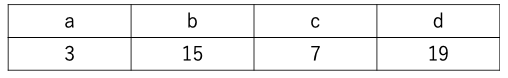
\includegraphics[width=9cm]{1wariate.png}
 % \caption{集合のハッシュ値表}
%\end{figure}


\begin{equation}
 \label{eq:datar}
h(A)=\min_{e \in \mbox{A}} \pi(e).
\end{equation}

さらに,Min-hashを用いたJaccard係数係数の近似計算を紹介する.
%元々,Min-Hashはハッシュテーブルを用いて,集合間類似検索を高速化することを目指して設計された一方で,
多数の要素を含む巨大な集合$A$のコンパクトな要約としてMin-Hashのハッシュ値を$k$個並べた\{$mh_1(A),mh_2(A),…,mh_k(A)$\}を使用するアプローチである.このMin-Hashのハッシュ値の集合を$A$のスケッチ \cite{Minhash}と呼ぶ.2つの集合$A$と$B$のスケッチ間で何個ハッシュ値が一致するかで $A $と$B$のハッシュ値を近似計算する.スケッチによって割り当てられる値はランダムに違うために,ハッシュ値もスケッチによって変わる.ハッシュ値が何個一致するかの確率はJaccard係数と一致するが,あくまで確率であるので,Min-Hashによるハッシュ値は近似値である.

\section{多重集合に対するMin-hash}
多重集合に対してMin-hashのハッシュ値を計算する手法を紹介する.文献では,大きく2つの方法が知られている.

(1)多重集合内の複数個のラベルに異なる値を割り当てる方法

(2)Consistent Weighted Sampling (CWS)  \cite{CWS} 

CWSは,Min-hashの出力の確率分布を模擬して,サンプリングすることでハッシュ値を計算する手法である.明示的に割り当て値を準備する必要がなく,多重集合が整数でなくても適用可能であるという利点がある.一方で確率の理論に精通していないと拡張が難しい手法でもある.(1)の同じラベルのアルファベットに異なる値を割り当てるやり方は多重集合の重みが整数であるという制約を受けるが,拡張は比較的容易な手法である.本論文では(1)の多重集合内の同一ラベルの要素に異なる値を割り当てる手法を使用する.

 
%多重集合において,集合の中に2つ以上同じアルファベットが存在することがある.多重集合に対するMin-Hashでは同一アルファベットに何個目かということに応じた異なる数値を割り当てる.

(1)のハッシュ値計算手法を例を用いて説明する.まず,図\ref{fig:2wariate}のように,アルファベット\{a,b,c,d\}に多重度が2である時の数値をランダムに割り当てる.
\begin{figure}[H]
  \centering
  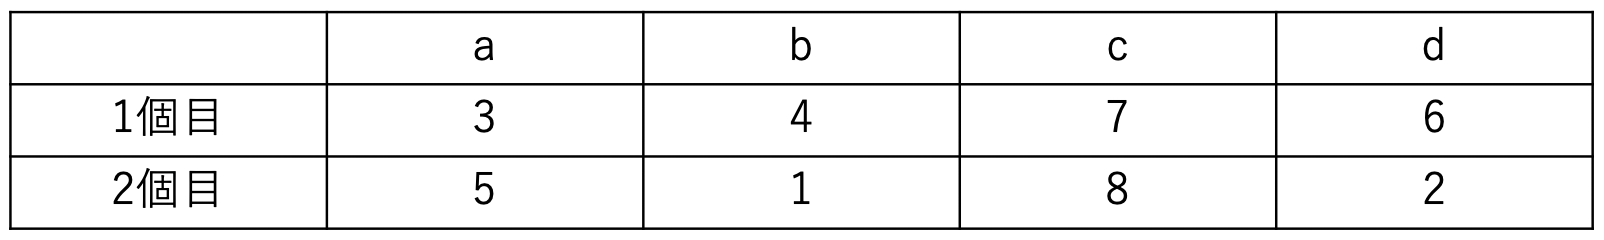
\includegraphics[width=15cm]{multi22.png}
  \caption{多重集合のハッシュ値表}
  \label{fig:2wariate}
\end{figure}

多重集合$A =\{a,b,b,c,c,d,d\}$とする.多重集合$A$に対して,図\ref{fig:2wariate}の割り当て表を用いて数値を割り当てる.そして,その中の最小値がMin-Hashによるハッシュ値となる(図\ref{fig:255}).

\begin{figure}[H]
  \centering
  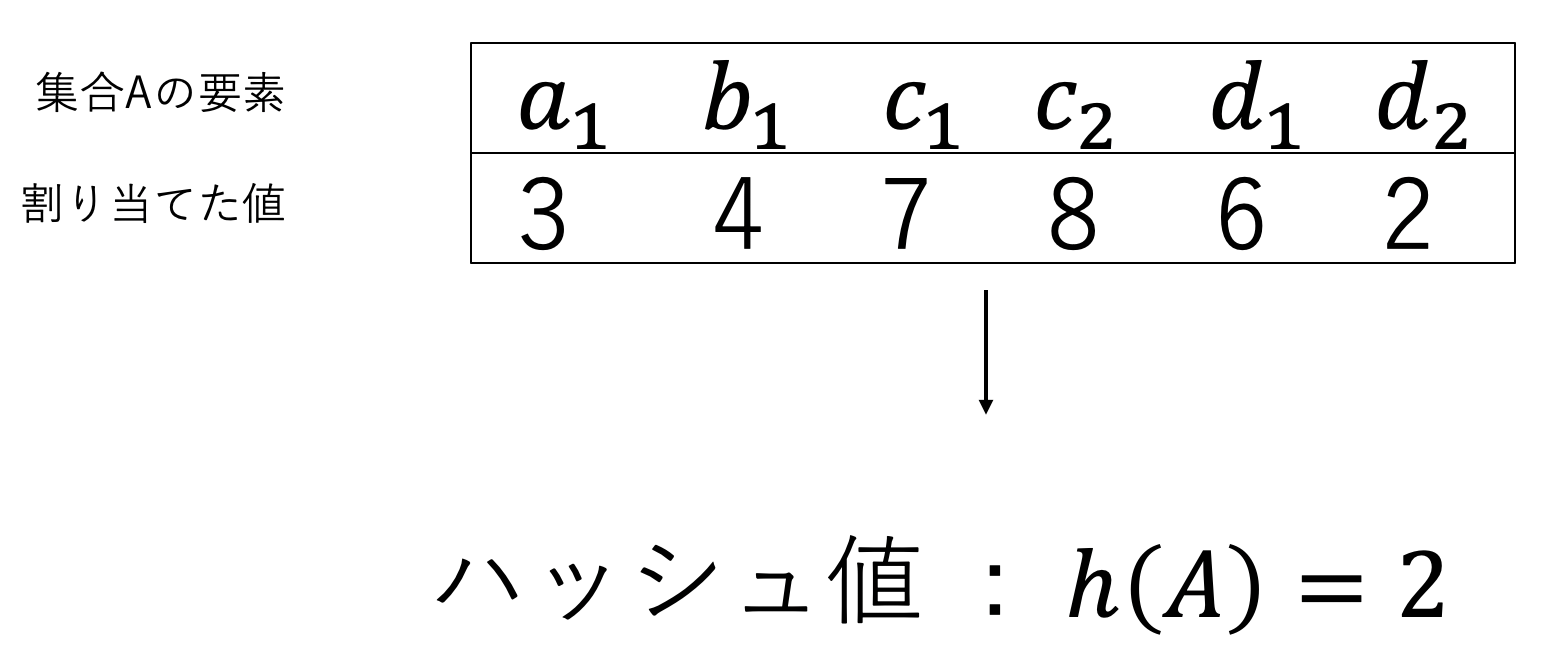
\includegraphics[width=15cm]{255.png}
  \caption{多重集合のハッシュ値計算}
  \label{fig:255}
\end{figure}

